\chapter{Results}

% **************************** Define Graphics Path **************************

\graphicspath{{Figs/}}

%********************************** % Section  **************************************

\section{Pixels} %Section - 1.1 
To understand what could be learnt from simulation data a simple first step was to convert hits in each layer of the VELO as an image. This is because convolutional neural networks (cnn's) are commonly used for image classification problems. The first task was to investigate whether a cnn could predict the output of a VELO layer, from the input of the previous VELO layer. Google's Tensorflow is the most popular machine learning library, however it can be difficult to use. Therefore Keras was used as a front-end to Tensorflow, this makes the process of creating the cnn model, training and testing much more intuitive. Before any data could be fed into a cnn the data had to be formatted correctly. To simulate a grid of pixels from the xyz coordinate data, the points were binned, with the number of bins representing the number of pixels in the x and y directions. The future VELO sensors are square 256x256 arrays of pixels, arranged 3 in a row, and 2 of these sensor triplets arranged in an L shape on each side of a module. To give relative realism to the binning process 1024 bins were used, giving an image with 1,048,576 total pixels. [Insert image of input layer]. However this method is very memory intensive and would crash Tensorflow when running on my laptop. Therefore the decision was made to down sample the image to 128x128 pixels, 16,384 total pixels. This would allow it to run while not impacting on the accuracy of the images formed, by this I mean down sampling did not lead to a situation where 2 hits ended up in the same pixel. 

\begin{figure}[h] % h for here in document
\centering
\begin{subfigure}[t]{0.45\textwidth}
\centering
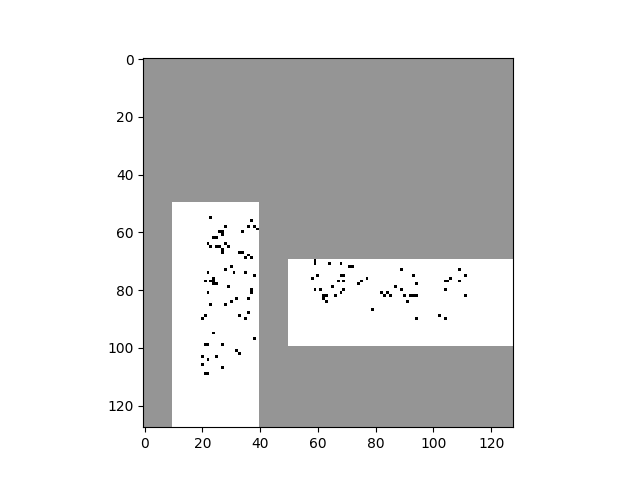
\includegraphics[width=\textwidth]{Figs/zeros.png}
\caption{} 
\label{fig:zeros} 
\end{subfigure}
~
\begin{subfigure}[t]{0.45\textwidth}
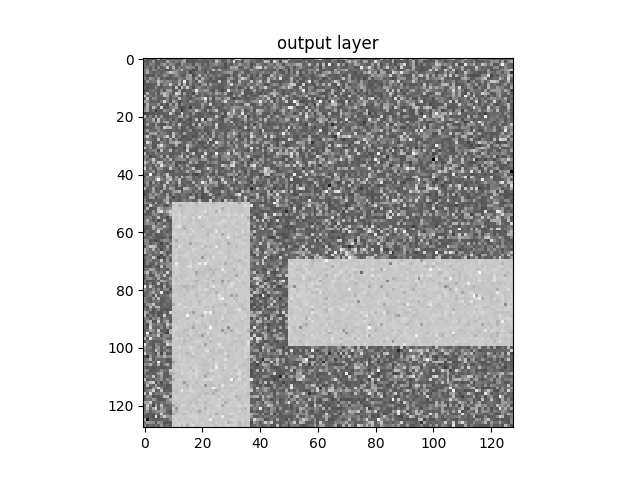
\includegraphics[width=\textwidth]{Figs/final_output0.png}
\caption{} 
\label{fig:final_output0}
\end{subfigure}
\end{figure}

\subsection{Results}
Various combinations of convolutional and fully connected layers were tried and tested but with few satisfactory results. There was promise as the network did start ‘learning’, ie the loss reduced over time. However on closer inspection it was found that the network was doing this by simply setting all output pixel values to 0. This reason for this is that the expected output of the cnn is a large array of 0's, with only a small number of 1's representing hits. Therefore if the accuracy is defined as the fraction of array elements are correct, then setting all 16,384 array elements to 0 will give >99\% accuracy when expecting 20 hits. An attempt to improve performance was made by designating which parts of the xy plane expected hits and which areas were not active pixel regions. This was done by changing the pixel values of active regions to be different. [Insert image of new input layer]. This had little effect on performance.

\subsection{Discussion}

%********************************** % Section  **************************************

\section{Points} %Section - 1.2
Very little success was had with this ‘pixel’ method therefore a different method was investigated. Instead of taking the xyz coordinates of each hit and turning it into an image, the raw xyz coordinates were used directly as inputs to a neural network. The method of formatting the data was as follows:
\begin{enumerate}
    \item Take the xyz coordinates for 2 modules of the detector, since Monte Carlo truth is known and given, remove any hits from particles that do not appear in both layers, this is helpful as it means we know which x and y points in 1 layer correspond to the xy points in the next module.
    \item  Create 1d arrays for the xy coordinates of each hit for every event in each simulation data file, each array has the format $(x0, y0, x1, y1, …, xn, yn)$. The hits from the first module are the data, the hits from the second layer are the labels of the neural network. Each array was split to create 6 final arrays: Training data, testing data, validation data, validation labels, testing data, testing labels. These were saved as datasets into an h5py file for fast reading and writing of data.
\end{enumerate}

It is very important to split data sets in this way. A critical rule of machine learning is that you cannot test a network on training data, this will lead to the network 'learning' the training data, known as overfitting. This will lead to a network which does not generalise to other data sets. Validation data sets are used in the training process to check the performance of a network. For most cases a split of 80\% training, 10\% validation and 10\% testing data is satisfactory.

The configuration of the neural network was different for this ‘points’ method. It was first thought that a problem with this method was that each event has a different number of hits, and neural networks need a consistent size input and output. The solution to this is to feed in one xy point at a time. So the network had input and output sizes of 2. This means 1 xy pair is trained on each time. The network had one fully connected hidden layer of size 1024.
The ‘points’ method has had promising results. For outer layers of the VELO it is very good at predicting hits in the next layer. But is less accurate for layers closer to the collision point. Figures \ref{fig:layers-136-161} and \ref{fig:layers-686-736}.

\begin{figure}[h] % h for here in document
\centering
\begin{subfigure}[t]{0.45\textwidth}
\centering
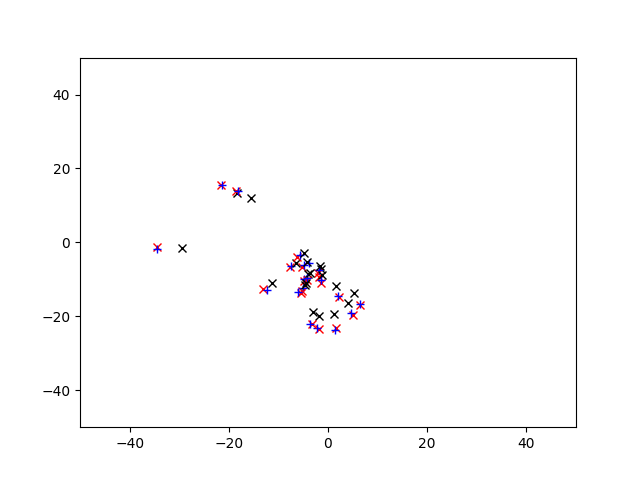
\includegraphics[width=\textwidth]{Figs/layers-136-161}
\caption{} 
\label{fig:layers-136-161} 
\end{subfigure}
~
\begin{subfigure}[t]{0.45\textwidth}
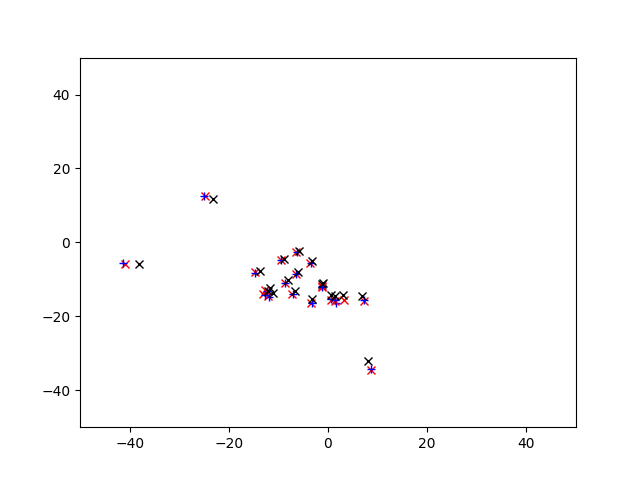
\includegraphics[width=\textwidth]{Figs/layers-686-736}
\caption{} 
\label{fig:layers-686-736}
\end{subfigure}
\end{figure}


\subsection{Results}

\subsection{Discussion}

%********************************** % Section  **************************************

\section{Closest numbers and points} %Section - 1.3
The next task was too create a neural network that could take a set of 8 random numbers as an input, and output the pair that have the smallest difference. This could then lead on to finding the closest pair of 2d points from a random set. The long term aim of this is to develop a system that can connect 2D points into tracks. 
Most effort was involved in creating data files in the correct format. Supervised learning requires labels that the neural network output can be tested against. A logical label would have the format of an array of zeros for each input number or vector, with a 1 value for the two points that are the closest together. With this problem solved it is a relatively simple job to setup a neural network model using Keras.

\subsection{Closest pairs of numbers}
Data set was 1 million sets of 8 random numbers between 0 and 1. This was trained using a fully connected Keras neural network with a structure of: 8 inputs for each random number, 8 outputs.
Binary cross entropy was used as a loss function. This means that each of the 8 output elements could be a number between 0 and 1. The last layer activation function was a sigmoid. Trained for 100 epochs. Figure .. shows the ROC curve for this method over the threshold. The use of a sigmoid final layer activation means each array element has a value between 0 and 1, the final prediction must be 0 or 1, therefore a threshold is set. Any element above this threshold is set to 1, otherwise is is set to 0. A ROC curve over this new parameter shows the best choice of the threshold. In this case it is 0.3.

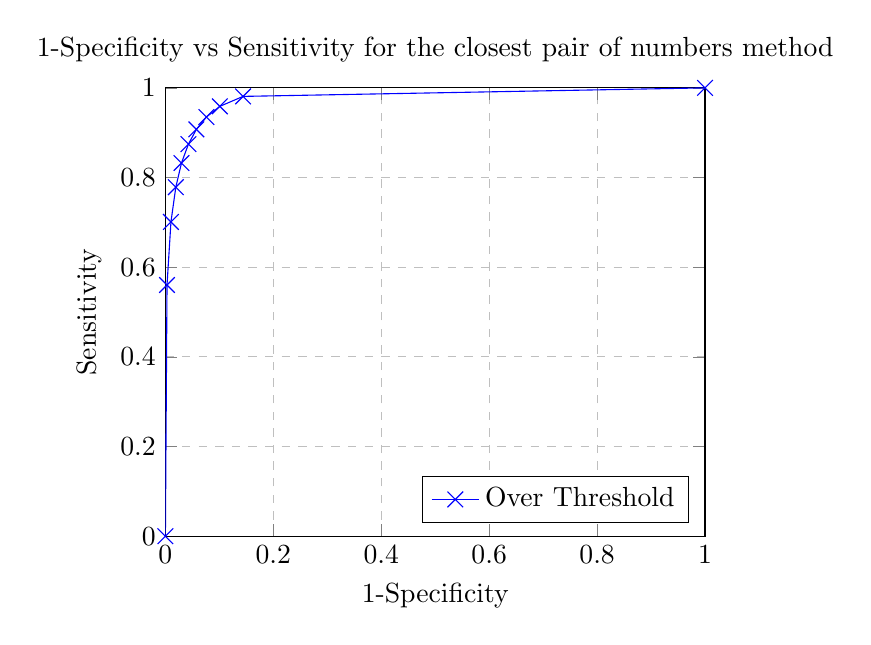
\begin{tikzpicture}[every mark/.append style={mark size=4pt}]
\begin{axis}[
    title={1-Specificity vs Sensitivity for the closest pair of numbers method},
    xlabel={1-Specificity},
    ylabel={Sensitivity},
    xmin=0, xmax=1,
    ymin=0, ymax=1,
    xtick={0,0.2,0.4,0.6,0.8,1},
    ytick={0,0.2,0.4,0.6,0.8,1},
    legend pos=south east,
    ymajorgrids=true,
    xmajorgrids=true,
    grid style=dashed,
]
 
\addplot[
    color=blue,
    mark=x,
    ]
    coordinates {
    (1,1)(0.1440,0.9810)(0.1009,0.9588)(0.0760,0.9349)(0.0574,0.9075)(0.0427,0.8745)(0.0298,0.8324)(0.0193,0.7785)(0.0103,0.701)(0.0030,0.5603)(0,0)
    };
    \legend{Over Threshold}
 
\end{axis}
\end{tikzpicture}


\subsection{Closest pairs of points}
Data set was 1 million sets of 10 random 2-vectors, with x and y ranging between 0 and 1. This was trained using a fully connected Keras neural network with a structure of: 20 inputs for the flattened array of points, 10 outputs.
Initial accuracy's of ~96\% for 1 million samples of random points were encouraging.
The accuracy of this method was tested further to fully understand the neural network output.

\begin{figure}[h] % h for here in document
\centering
\begin{subfigure}[t]{0.45\textwidth}
\centering
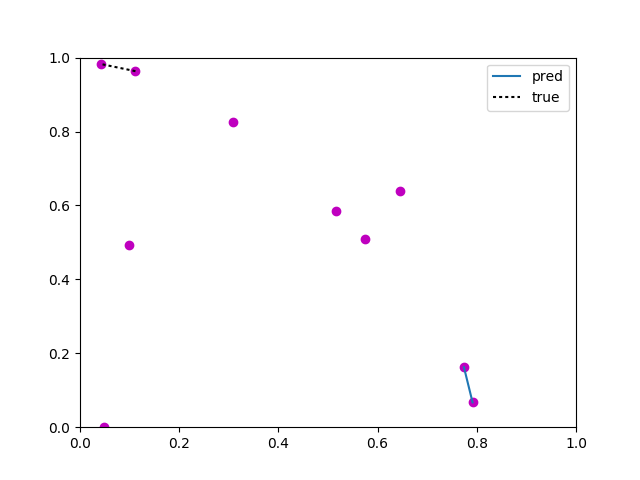
\includegraphics[width=\textwidth]{Figs/closest_dist_fail2}
\caption{An example of a failure case} 
\label{fig:closest_dist_fail2} 
\end{subfigure}
~
\begin{subfigure}[t]{0.45\textwidth}
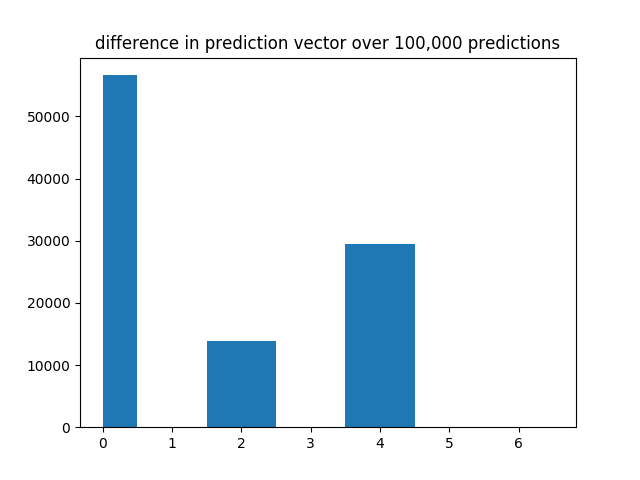
\includegraphics[width=\textwidth]{Figs/pred_dif_hist}
\caption{A histogram representing the output of the neural network} 
\label{fig:pred_dif_hist}
\end{subfigure}
\end{figure}

The output of the neural network was a vector of zeros with length 10. Two 1's in this vector represent the two points to be connected. If there was a 1 at position 2 and position 4 then points 2 and 4 were deemed the closest pair.

\[
\begin{pmatrix}
0 & 0 & 1 & 0 & 1 & 0 & 0 & 0 & 0 & 0
\end{pmatrix}
\]

To investigate the output of the network the difference between the predicted and true vectors was calculated. This was done by taking the absolute of element wise subtraction. Therefore if the predicted vector was the same as the true vector then the difference would be 0. If one point was incorrectly classified then the difference would be 2. And finally if both points were incorrectly classified then the difference would be 4. The histogram in Figure \ref{fig:pred_dif_hist} shows this over all 100000 testing samples. The majority are correctly classified (57\%), some have one incorrect classification (14\%) and some have two incorrect classifications (29\%). These numbers are nowhere near the 96\% claimed accuracy, this does not mean however, that the network is bad at finding pairs of closest points. Failure cases were investigated to understand. Figure \ref{fig:closest_dist_fail2} a shows one failure case. The neural network has found a pair of points with a distance apart very close to the true closest pair. For the intended application in particle physics this is a very satisfactory result.


%********************************** % Section  **************************************

\section{Joining the dots} %Section - 1.4 
After initial success of finding the two closest points I moved onto connecting more points together to 'join the dots'. This was defined as finding the two closest points as before, then from one of these points finding the next closest. This was achieved by using the neural network to calculate the adjacency matrix of the points.\\
Finding the two closest points is an established problem which can be solved quickly.\\
The next step was to use the neural network for the entire process, finding the two closest points and then joining the dots. It was important to find the correct way to represent the connections between points. Many different ways were tried. Firstly using the adjacency matrix of the points, then using the indices of the points was tried, also simply using the network to give back the coordinates in the connected order.\\
Only one method worked well. that was to train the neural network to output the undirected adjacency matrix of the points. An adjacency matrix is an n x n matrix, for n points, which shows which points are connected to each other. There are 0's where there is no connection, and 1's where there is a connection. So, for example, if points 2 and 3 are connected, there will be a 1 in the 2nd row and 3rd column of the adjacency matrix. However there will also be a 1 in the 3rd row and 2nd column, as the direction of the connection is not important. It was also found that the network's performance improved when the upper or lower triangle of the matrix is removed.

\[
\begin{pmatrix}
0 & 0 & 0 & 0 \\
0 & 0 & 0 & 0 \\
0 & 0 & 0 & 1 \\
0 & 0 & 1 & 0
\end{pmatrix}
\]

The neural network was fed sets of 10 random 2d points with x and y ranging between 0 and 1. The adjacency matrix for each set of 10 points was calculated. To start 1 million sets of random numbers were used, 80\% for training, 10\% for validation and 10\% for testing. After initial testing gave encouraging results 5 million sets of random numbers and corresponding adjacency matrices were generated.\\
Here I will include results.

\section{Receiver Operating Codes (ROC)}
Results must have an error metric so that they can be compared. The language of receiver operating codes fits well in this context. The true connections between points are calculated so that the neural networks can be trained. Therefore the neural network output can be correct or incorrect in these ways:
\begin{itemize}
    \item True Positive (TP) - A connection was made when it should have been.
    \item True Negative (TN) - A connection was not made when it should not have been.
    \item False Positive (FP) - A connection was made when it should not have been.
    \item False Negative (FN) - A connection was not made when it should have been.
\end{itemize}
To understand the numbers of these outcomes the Sensitivity and Specificity are calculated.
\[ Sensitivity = \frac{TP}{TP + FN} \]
\[ Specificity = \frac{TN}{TN + FP} \]

Both these metrics must be high in order to have satisfactory results. If the sensitivity is high but the specificity is low then this indicates the neural network is connecting all points together, this will make sure all correct connections are made. If the specificity is high but the sensitivity is low then the network will not connect any points together. Therefore a balance is needed for good performance\\
A ROC curve is a plot of Sensitivity against 1-Specificity over some parameter. In my case the parameter was the threshold of the neural network output. Thanks to the last layer having a Sigmoid activation function each element of the output was a number between 0 and 1. The adjacency matrix must only contain 0's and 1's so a threshold was used, any output element below the threshold was set to 0, and any element above the threshold was set to 1. Plotting the ROC curve allows for tuning of the threshold to an optimum. The further to the top and left the ROC curve goes indicates better performance.
Compare definition of sensitivity & specifity and efficiency & purity.

\begin{figure}[h] % h for here in document
\centering
\begin{subfigure}[t]{0.45\textwidth}
\centering
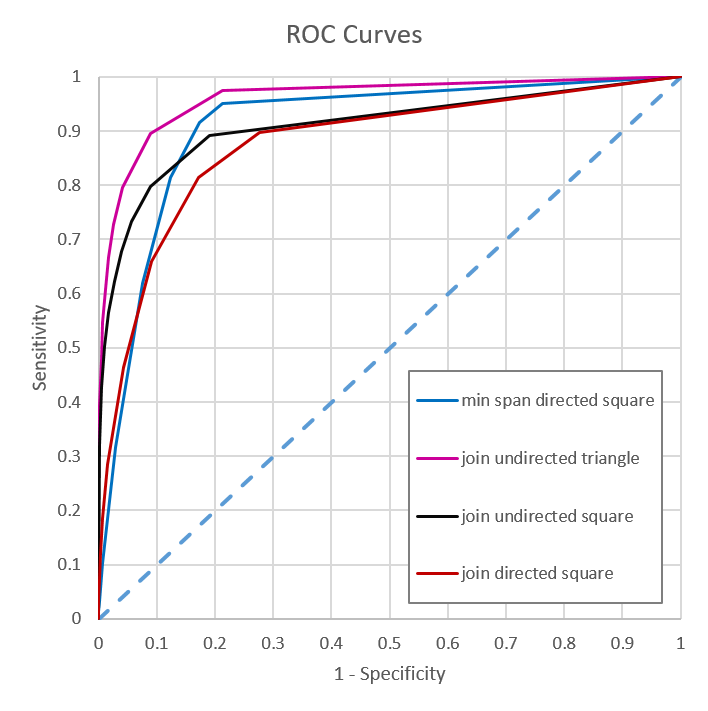
\includegraphics[width=\textwidth]{Figs/ROC_2.png}
\caption{ROC curve for different methods of 'joining the dots'} 
\label{fig:ROC_2} 
\end{subfigure}
~
\begin{subfigure}[t]{0.45\textwidth}
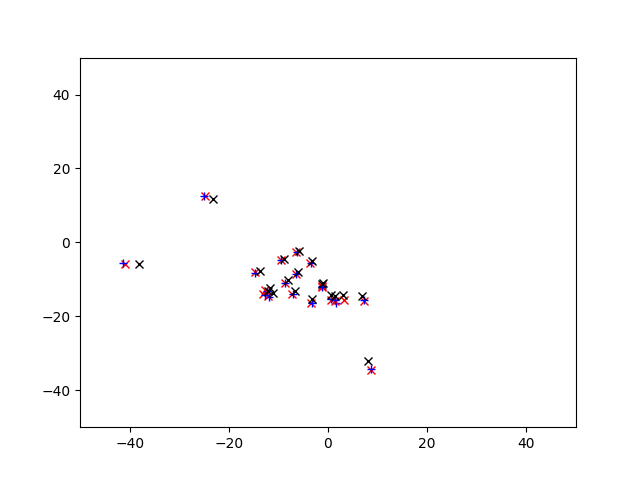
\includegraphics[width=\textwidth]{Figs/layers-686-736}
\caption{} 
\label{fig:layers-686-736}
\end{subfigure}
\end{figure}

\subsection{Results}

\subsection{Discussion}